\documentclass{standalone}
\usepackage{bm}
% \newcommand{\bm}[1]{\boldsymbol{\mathbf{#1}}}
\usepackage{tikz}
\usetikzlibrary{calc}
\usetikzlibrary{angles,quotes}


\begin{document}
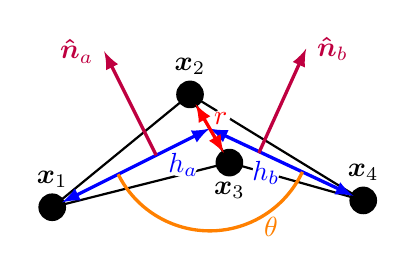
\begin{tikzpicture}[x=2cm, y=2cm, z={(0.25,-0.433)}, >=latex]
  % Nodes
  \node[label=$\bm{x}_1$] (x1) at (0, 0, 0) {};
  \node[label=$\bm{x}_2$] (x2) at (1, 0.5, -0.5) {};
  \node[label=below:$\bm{x}_3$] (x3) at (1, 0.5, 0.5) {};
  \node[label=$\bm{x}_4$] (x4) at (2, 0, -0.1) {};
  \fill (x1) circle (5pt);
  \fill (x2) circle (5pt);
  \fill (x3) circle (5pt);
  \fill (x4) circle (5pt);

  % Bonds
  \draw[thick] (x1) -- (x2);
  \draw[thick] (x1) -- (x3);
  \draw[thick] (x2) -- (x3);
  \draw[thick] (x2) -- (x4);
  \draw[thick] (x3) -- (x4);

  % Heights
  \coordinate (x23) at ($(x2)!0.5!(x3)$);
  \draw[<->,blue,very thick] (x23) -- node[label={[fill=white,inner sep=0pt,rounded corners=4pt,shift={(0.3,-0.15)}]$h_a$}] {} (x1);
  \draw[<->,blue,very thick] (x23) -- node[label={[fill=white,inner sep=0pt,rounded corners=4pt,shift={(-0.1,-0.22)}]$h_b$}] {} (x4);

  % Bond length
  \draw[<->,red,very thick] (x2) -- node[above right,fill=white,inner sep=1pt,rounded corners=4pt] {$r$} (x3);

  % Normals
  \coordinate (na0) at ($0.33*(x1)+0.33*(x2)+0.33*(x3)$);
  \coordinate (nb0) at ($0.33*(x2)+0.33*(x3)+0.33*(x4)$);
  \coordinate (na1) at ($ (na0)!1!-90:(x1) $);
  \coordinate (nb1) at ($ (nb0)!1!90:(x4) $);
  \draw[->,purple,very thick] (na0) -- (na1) node[left] {$\bm{\hat{n}}_a$};
  \draw[->,purple,very thick] (nb0) -- (nb1) node[right] {$\bm{\hat{n}}_b$};

  % Angle
  \pic [draw,"$\theta$"{shift=(18:0.4)},orange,very thick,angle radius=1.3cm,angle eccentricity=1.15] {angle = x1--x23--x4};
\end{tikzpicture}
\end{document}
